\documentclass[tikz]{standalone}
\usepackage{tikz}
\usetikzlibrary{positioning, graphs}
\usetikzlibrary{graphs.standard}
\begin{document}
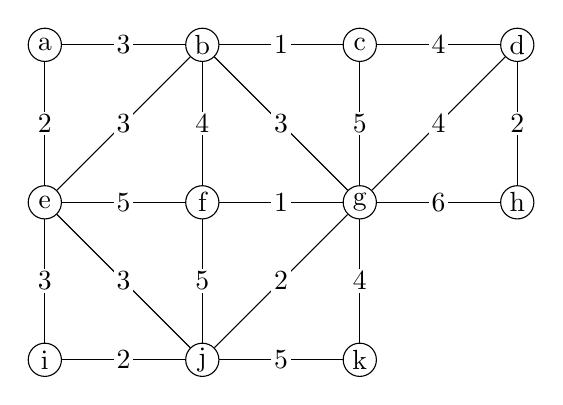
\begin{tikzpicture}
\begin{scope}
    [vertex/.style={draw,circle,inner sep = 0em, minimum size = 1.2em},
        edgelabel/.style = {fill = white, inner sep = 0.1em}]
    \node[vertex] (a) at (0,0) {a};
    \node[vertex] (b) at (2,0) {b};
    \node[vertex] (c) at (4,0) {c};
    \node[vertex] (d) at (6,0) {d};
    \node[vertex] (e) at (0,-2) {e};
    \node[vertex] (f) at (2,-2) {f};
    \node[vertex] (g) at (4,-2) {g};
    \node[vertex] (h) at (6,-2) {h};
    \node[vertex] (i) at (0,-4) {i};
    \node[vertex] (j) at (2,-4) {j};
    \node[vertex] (k) at (4,-4) {k};
    
    \draw[-] (a) to node[edgelabel]{$3$} (b);
    \draw[-] (a) to node[edgelabel]{$2$} (e);
    \draw[-] (b) to node[edgelabel]{$3$} (e);
    \draw[-] (b) to node[edgelabel]{$4$} (f);
    \draw[-] (b) to node[edgelabel]{$3$} (g);
    \draw[-] (b) to node[edgelabel]{$1$} (c);
    \draw[-] (c) to node[edgelabel]{$5$} (g);
    \draw[-] (c) to node[edgelabel]{$4$} (d);
    \draw[-] (d) to node[edgelabel]{$4$} (g);
    \draw[-] (d) to node[edgelabel]{$2$} (h);
    \draw[-] (e) to node[edgelabel]{$5$} (f);
    \draw[-] (f) to node[edgelabel]{$1$} (g);
    \draw[-] (g) to node[edgelabel]{$6$} (h);
    \draw[-] (e) to node[edgelabel]{$3$} (i);
    \draw[-] (e) to node[edgelabel]{$3$} (j);
    \draw[-] (f) to node[edgelabel]{$5$} (j);
    \draw[-] (g) to node[edgelabel]{$2$} (j);
    \draw[-] (g) to node[edgelabel]{$4$} (k);
    \draw[-] (i) to node[edgelabel]{$2$} (j);
    \draw[-] (j) to node[edgelabel]{$5$} (k);
\end{scope}
\end{tikzpicture}
\end{document}